\chapter{Anwendungen}
\label{chp:applications}
Um den Aufwand für die spätere Benutzung zu reduzieren ist zuerst eine allgemeine Implementation des \textsc{ESN}s geschrieben worden. 

\section{Vorhersage eines Rössler-Systems}
Eine erste Anwendung um die Möglichkeiten eines \textsc{ESN} zu demonstrieren besteht in der Vorhersage des Verhaltens eines \textit{Rössler-Systems}
\begin{align}
\label{eq:application_roessler_pde}
\begin{split}
\dot{x} &= -(y+z)\\
\dot{y} &= x + 0.25 \cdot  y\\
\dot{z} &= 0.4 + (x - 8.5)\cdot z.
\end{split}
\end{align}

Hierbei werden zwei verschiedene Aufgaben betrachtet: \textit{(a)} die Vorhersage von $x(n+50)$ durch die Kenntnis von $x(n)$ und \textit{(b)} die Kreuz-Vorhersage $y(n)$ durch $x(n)$. Für beide Aufgaben wurde das System für jeweils $10000$ Schritte mit einer Abtastrate $\Delta t = 0.05$ simuliert, wobei die Hälfte der Daten für das Training und der Rest für die Testergebnisse verwendet worden ist.

\subsection{Vorhersage $x(n) \rightarrow x(n+48)$}
Hierfür ist durch eine \textsc{GridSearch} ein geeignetes System gefunden werden, Parameter in der Tabelle \ref{tab:application_roessler} dargestellt sind. Als Maß für die Optimierung wurde der \textit{Mean Square Error (MSE)} benutzt.

Hierbei wurde für den Trainingsvorgang ein Fehler $MSE = 0.575$ und für den Testvorgang von $MSE = 0.270$ bestimmt. Ein grafischer Vergleich zwischen der dem Signal $y(t)$ und der Vorhersage $v(n)$ ist in Abbildung \ref{fig:application_roessler_a} zu finden.

\begin{table}[H]
	\centering
	\captionsetup{width=0.9\linewidth}
		\begin{tabular}{|c|c|c|}
		\rule[-1ex]{0pt}{3.5ex} Variable & \hspace{4ex} Wert für \textit{(a)} \rule[-1ex]{4ex}{0pt} & \hspace{4ex} Wert für \textit{(b)} \rule[-1ex]{4ex}{0pt}\\ 
		\hline \hline 
		\rule[-1ex]{0pt}{3.5ex} $N$ & $300$ & $500$ \\ 
		\hline 
		\rule[-1ex]{0pt}{3.5ex} $\alpha$ & $0.10$ & $0.20$ \\ 
		\hline 
		\rule[-1ex]{0pt}{3.5ex} $\rho(|\mathbf{W}|)$ & $0.035$ & $0.01$\\ 
		\hline 
		\rule[-1ex]{0pt}{3.5ex} $\nu_{max}$ & $0.01$ & $0.01$\\ 
		\hline 
	\end{tabular} 
	\caption{Auflistung der Parameter für das jeweilige \textsc{ESN} für (a) und (b).}
	\label{tab:application_roessler}
\end{table}

\vspace{-4ex}
\begin{figure}[H]
    \centering
    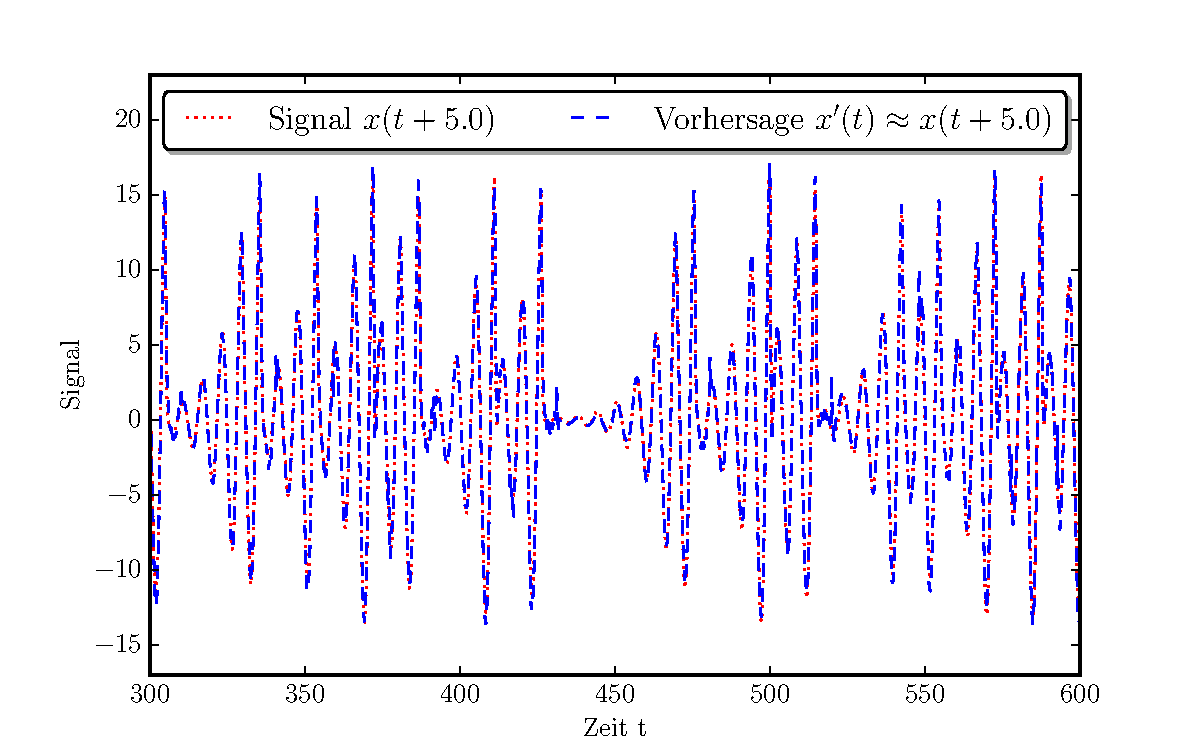
\includegraphics[width = 0.9 \textwidth]{figures/roessler_pred50.pdf}
    \caption{Graphische Darstellung des Signals $y(n)$ und der Vorhersage $y(n+50)$.}
    \label{fig:application_roessler_a}
\end{figure}



\subsection{Kreuz-Vorhersage $x(n) \rightarrow y(n)$}
Auch hierfür konnte sehr schnell durch eine \textsc{GridSearch} ein geeignetes System gefunden werden. Als Maß wurde ebenfalls der \textit{MSE} benutzt. Die gefundenen Parameter sind ebenfalls in der Tabelle \ref{tab:application_roessler} dargestellt.\\
Für das Auslesen wurde eine Linearkombination genutzt, wobei die Lösung $\mathbf{W}_{out}$ mittels der Pseudoinversen bestimmt worden ist.\\

Hierbei wurde für den Trainingsvorgang ein Fehler $MSE_{train} = 0.011$ und für den Testvorgang von $MSE_{test} = 0.091$ bestimmt. Die grafische Darstellung der Vorhersage $v(n)$ und des ermittelten Fehlers sind in den Abbildungen \ref{fig:application_roessler_b1} zu finden. Im Vergleich zu anderen Publikationen \cite{parlitz2005} ergibt sich ein ähnlicher Fehler. Leider kann hierbei nur mit den Graphen verglichen werden, da keine Fehler angegeben sind.

\begin{figure}[H]
    \centering
     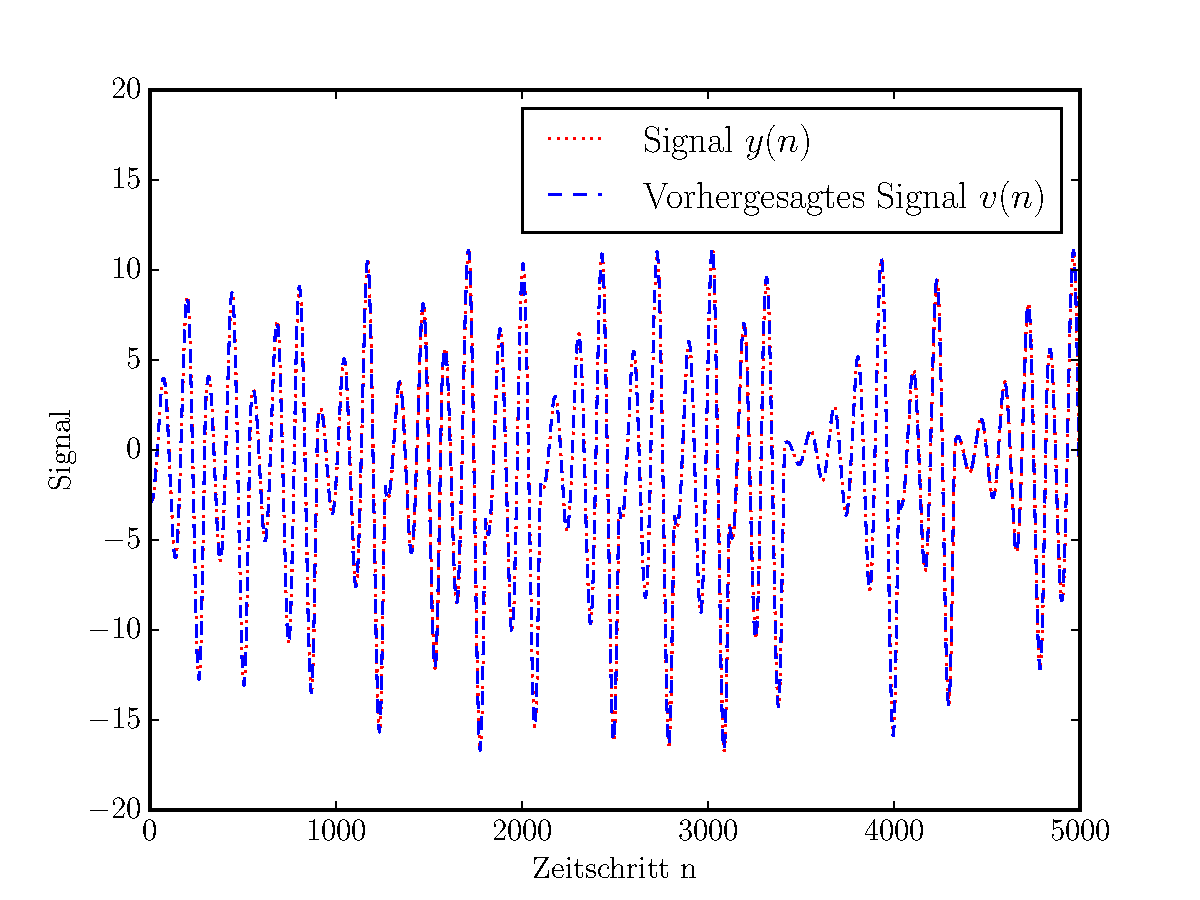
\includegraphics[width = 0.9 \textwidth]{figures/roessler_cross_pred.pdf}
     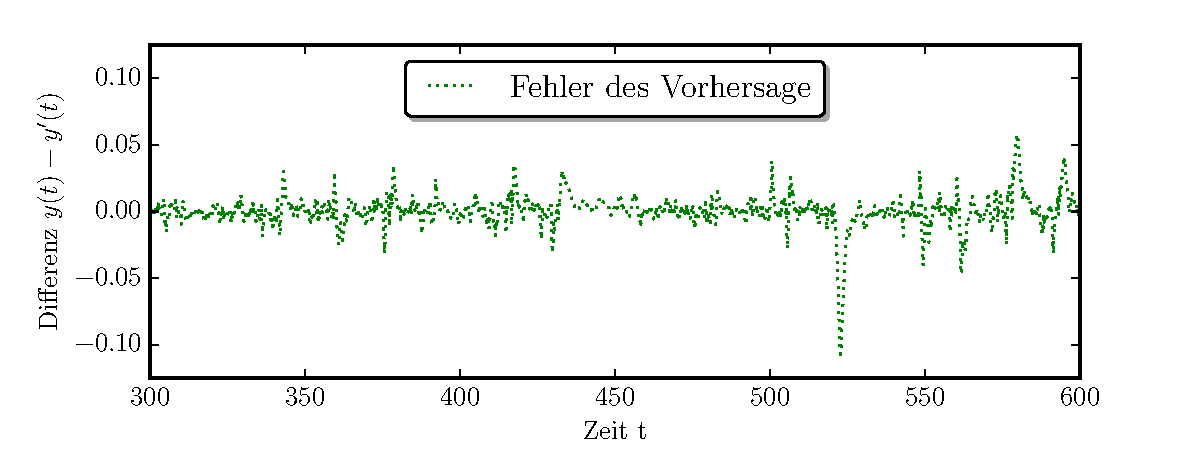
\includegraphics[width = 0.9 \textwidth]{figures/roessler_cross_err.pdf}
    \caption{Graphische Darstellung des Signals $y(n)$, der Vorhersage $v(n)$ und des Fehlers $y(n)-v(n)$.}
    \label{fig:application_roessler_b1}
\end{figure}

\section{Vorhersage eines Mackey-Glass-Systems}
Als nächste Anwendung wird ein \textit{Mackey-Glass-System}
\begin{align}
\label{eq:application_roessler_pde}
\begin{split}
\dot{x}(t) &= \beta \frac{x(t-\tau)}{1+x(t-\tau)^n}-\gamma x(t)\\
\end{split}
\end{align}
betrachtet, wobei $\tau = 17, n=10, \beta = 0.2$ gewählt wurden. Dies ist eine beliebte Aufgabe im Bereich der Vorhersagen chaotischer Zeitreihen.\\
Für dieses System wurde in Analogie zu  \citep{caraballo2014} die Vorhersage $x(n) \rightarrow x(n+84)$ betrachtet, wobei die Parameter aus Tabelle \ref{tab:application_mackeyglass} genutzt wurden. Hierfür wurden mittels der \textit{Euler-Diskretisierung} Werte für $0 \leq t \leq 4000$ simuliert, wobei die ersten $2000$ Werte für den Trainings und die anderen für den Test-Vorgang genutzt wurden. Es wurde zur Lösung die \textit{Tikhonov Regularisierung} benutzt.

\begin{table}[H]
	\centering
		\begin{tabular}{|c|c|}
		\rule[-1ex]{0pt}{3.5ex} Variable & \hspace{4ex} Wert \rule[-1ex]{4ex}{0pt}\\ 
		\hline \hline 
		\rule[-1ex]{0pt}{3.5ex} $N$ & $1000$ \\ 
		\hline 
		\rule[-1ex]{0pt}{3.5ex} $\alpha$ & $0.20$ \\ 
		\hline 
		\rule[-1ex]{0pt}{3.5ex} $\rho(\mathbf{W})$ & $1.25$ \\ 
		\hline 
		\rule[-1ex]{0pt}{3.5ex} $\nu_{max}$ & $\num{1e-4}$ \\ 
		\hline 
		\rule[-1ex]{0pt}{3.5ex} $\beta$ & $\num{1e-8}$ \\ 
		\hline 
	\end{tabular} 
	\caption{Auflistung der benutzten Parameter des \textsc{ESN}.}
\label{tab:application_mackeyglass}
\end{table}

Interessant ist, dass der Spektralradius größer $1.0$ ist - dies ist möglich, da ein konstanter \textit{Bias} von $1.0$ als weiteres Eingangssignal genutzt wurde.\\
Eine Darstellung der Ergebnisse ist in Abbildung \ref{fig:application_mackeyglass} zu sehen. Hierbei wurde der \textit{MSE} für die gesamte Trainingsphase als $MSE_{train} = 0.0042$ und der der Testphase als $MSE_{test} = \num{9e-5}$ bestimmt.

\begin{figure}[H]
    \centering
    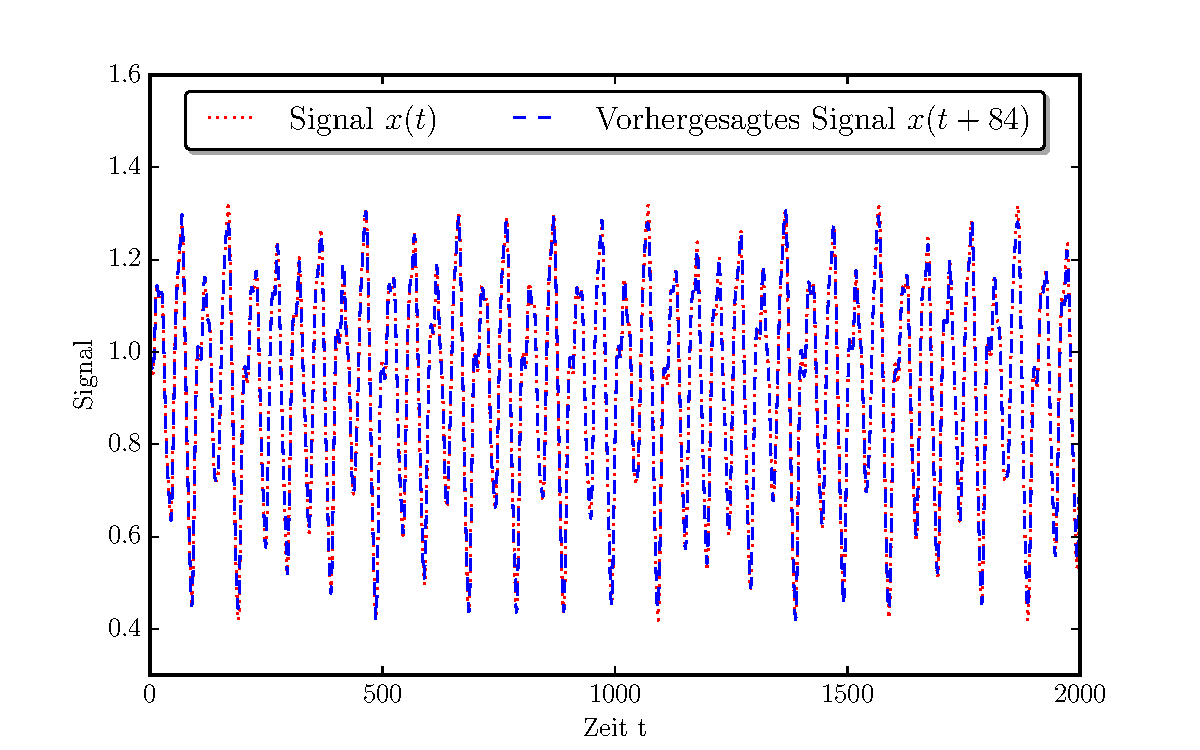
\includegraphics[width = 0.9 \textwidth]{figures/mackeyglass_pred.pdf}
    \caption{Graphische Darstellung des Signals $x(t)$ und der Vorhersage $x(t+84)$.}
    \label{fig:application_mackeyglass}
\end{figure}

Dies ist eine starke Verbesserung im Vergleich zu dem besten Ergebnis aus \citep{caraballo2014} mit $MSE = 0.0014$, wobei anzumerken ist, dass dort eine kleinere Trainings- und Testphase gewählt worden ist.